\section{Theoretical Analysis}
\label{sec:analysis}
\indent

In this section, the circuit shown in Figure \ref{fig:rc} is analysed theoretically.

This circuit has 4 meshes, in which we assume the current flows clockwise (Figure \ref{fig:mesh}), and 8 nodes (Figure \ref{fig:Nodes}).

The voltage source $v_s$ has a voltage of $V_s$ for $t\leq0$.
For $t>0$ its voltage varies with time according to equation \ref{eq:vs}.

\begin{figure}[H] \centering
    \includegraphics[width=0.7\linewidth]{t2_meshLabels.pdf}
    \caption{Current flow on each mesh.}
    \label{fig:mesh}
\end{figure}

\begin{figure}[H] \centering
    \includegraphics[width=0.7\linewidth]{t2_nodeLabels.pdf}
    \caption{Nodes and their respective labels.}
    \label{fig:Nodes}
\end{figure}




\subsection{Circuit analysis for $t<0$}
\label{subsection:circ_analysis}

\indent

For $t<0$, $v_s=V_s$ and the capacitor acts like an open circuit ($I_c=0$) since it is fully charged. 

There are 8 nodes in total which means that we need 8 linearly independent equations to find out the voltages in each node and solve the circuit. Therefore, we use the Kirchhoff Current Law (KCL, shown in equation \ref{eq:KCL}) in every node that is not connected to a voltage source (nodes 2, 3, 6 and 7, which are identified in Figure~\ref{fig:rc}).

\begin{equation}
    \sum_{k=1}^{n} I_k = 0.
    \label{eq:KCL}
\end{equation}

Node 4 (the reference node) is connected to the ground, which means that its voltage ($V_0$) is 0. 

It is also known that the value of a voltage source is equivalent to the difference of the voltages in each node to which the source is connected. That allows us to create two more equations, since there are two voltage sources in the circuit.

For the $8^{th}$ equation we can create a \textit{supernode} with nodes 5 and 8, since the dependent voltage source is not connected to the reference node. Through this method, nodes 5 and 8 are regarded as one single node (a \textit{supernode}) by ignoring the voltage source between them.

To demonstrate the process, the node 2 equation resulting from the KCL application is the following:

\begin{equation}
    (V_2-V_3)\cdot G_2=(V_5-V_2)\cdot G_3+(V_1-V_2)\cdot G_1.
    \label{n2}
\end{equation}

Doing this on all possible nodes/supernode and adding the extra equations, regarding the voltage sources, a system of linear equations can be obtained and solved with the aid of \textit{Octave}. The results are presented on table~\ref{tab:Volts}.

\begin{table}[H]
  \centering
  \begin{tabular}{|l|r|}
    \hline    
    {\bf Name} & {\bf Value [V]} \\ \hline
    V1 & 5.008942 \\ \hline 
V2 & 4.808960 \\ \hline 
V3 & 4.394159 \\ \hline 
V4 & 0.000000 \\ \hline 
V5 & 4.837862 \\ \hline 
V6 & 5.474755 \\ \hline 
V7 & -2.008723 \\ \hline 
V8 & -2.970917 \\ \hline 

  \end{tabular}
  \caption{Results from the node analysis, from \textit{Octave}.}
  \label{tab:Volts}
\end{table}

While analysing the current in each mesh we used the Kirchhoff Voltage Law (KVL, shown in equation \ref{eq:KVL}) in every mesh. However, it would be equivalent to use Ohm's law (equation \ref{eq:OL}) since we already know the resistance of each resistor and the voltage at every node. The results of this analysis are shown in table \ref{tab:currents}.

\begin{equation}
    \sum_{k=1}^{n} V_k = 0 \hspace{5pt},
    \label{eq:KVL}
\end{equation}

\begin{equation}
    R=\frac{V}{I} \hspace{5pt}.
    \label{eq:OL}
\end{equation}

\begin{table}[H]
  \centering
  \begin{tabular}{|l|r|}
    \hline    
    {\bf Name} & {\bf Value [A]} \\ \hline
    Ia & 0.194523 \\ \hline 
Ib & -0.204136 \\ \hline 
Ic & 0.961761 \\ \hline 
Id & 0.000000 \\ \hline 

  \end{tabular}
  \caption{Results from the mesh analysis, from \textit{Octave}.}
  \label{tab:currents}
\end{table}

Since we know the current on each mesh we can compute the current on every branch with the aid of KCL (equation \ref{eq:KCL}). The results can be seen in table \ref{tab:Bcurrents}. 

\begin{table}[H]
  \centering
  \begin{tabular}{|l|r|}
    \hline    
    {\bf Name} & {\bf Value [A]} \\ \hline
    Ib & -0.204136 \\ \hline 
Id & 0.000000 \\ \hline 
R1 & 0.194523 \\ \hline 
R2 & -0.204136 \\ \hline 
R3 & -0.009613 \\ \hline 
R4 & 1.156284 \\ \hline 
R5 & 0.204136 \\ \hline 
R6 & 0.961761 \\ \hline 
R7 & 0.961761 \\ \hline 

  \end{tabular}
  \caption{Results from mesh analysis, using \textit{Octave}.}
  \label{tab:Bcurrents}
\end{table}


\subsection{Circuit analysis for a voltage source-equivalent capacitor}

\indent

Studying the circuit with the capacitor acting as a voltage source is equivalent to studying the circuit for $t=0$. As stated, the independent voltage source has a voltage of 0 volts and therefore is equivalent to a conductor wire on a closed circuit. Knowing this, it is possible to obtain the equivalent resistance of the circuit, and, therefore, obtain $\tau$ (the time constant of the capacitor).

A node analysis was performed similarly to what was done before. The capacitor voltage ($V_x$) was defined as $V_x = V_6-V_8$, where $V_6$ and $V_8$ are the voltages in node 6 and 8, respectively, obtained on the first analysis (\ref{subsection:circ_analysis}). The results are expressed in table \ref{tab:Volts2}.


\begin{table}[H]
  \centering
  \begin{tabular}{|l|r|}
    \hline    
    {\bf Name} & {\bf Value [V]} \\ \hline
    \input{../Analysis/Voltages_2.tex}
  \end{tabular}
  \caption{Results obtained from node analysis, using \textit{Octave}.}
  \label{tab:Volts2}
\end{table}

Once again, the currents are calculated similarly to the previous section and are presented on the following table (table \ref{tab:Bcurrents2}):

\begin{table}[H]
  \centering
  \begin{tabular}{|l|r|}
    \hline    
    {\bf Name} & {\bf Value [A]} \\ \hline
    \input{../Analysis/BranchCurrents_2.tex}
  \end{tabular}
  \caption{Results obtained from mesh analysis, using \textit{Octave}.}
  \label{tab:Bcurrents2}
\end{table}


Here, we establish an equivalence between the capacitor and a voltage source, in order to compute the equivalent resistance ($R_{eq}$). $R_{eq}$ is the scalar resistance value obtained by substituting the entire circuit by a single voltage source and a single resistor, connected in series, via \emph{Thévenin's Equivalence Theorem}. To calculate this scalar, we divide the voltage differential on the capacitor and its current to obtain the resistance, using Ohm's Law (\ref{eq:OL}).

With the aid of this new information, it is possible to calculate the time constant ($\tau$). For a RC circuit, the time constant can be obtained from the following equation (\ref{eq:tau}):

\begin{equation}
    \tau = R_{eq}\cdot C
    \label{eq:tau}
\end{equation}

The results for $R_{eq}$ and $\tau$ are present on the table \ref{tab:Req}:

\begin{table}[H]
  \centering
  \begin{tabular}{|l|r|}
    \hline    
    {\bf Name} & {\bf Value} \\ \hline
    \input{../Analysis/Req-tau.tex}
  \end{tabular}
  \caption{$R_{eq}$ (in $\Omega$) and $\tau$ (in s), from \textit{Octave}.}
  \label{tab:Req}
\end{table}

\subsection{Circuit analysis for $t>0$}
\subsubsection{Transient analysis: Natural solution}

As a result from the previous analysis (table \ref{tab:Bcurrents2}) we know that $V_8=0$ and therefore $V_x=V_6$.

Knowing that this circuit only contains one capacitor and all the other components are resistors and voltage/current sources, the voltage of the capacitor ($v_x$) can be given by equation \ref{eq:vx}:

\begin{equation}
    v_x(t)=v_x(+\infty)+[v_x(0)-v_x(+\infty)]e^{-\frac{t}{\tau}} \hspace{5pt},
    \label{eq:vx}
\end{equation}
where $v_x(0)=V_x=V_6-V_8$ and $v_x(+\infty)=0$, since the capacitor will tend to discharge completely over time.

With this, we can plot $V_6$, as seen in image \ref{fig:NatOc}:


\begin{figure}[H] \centering
    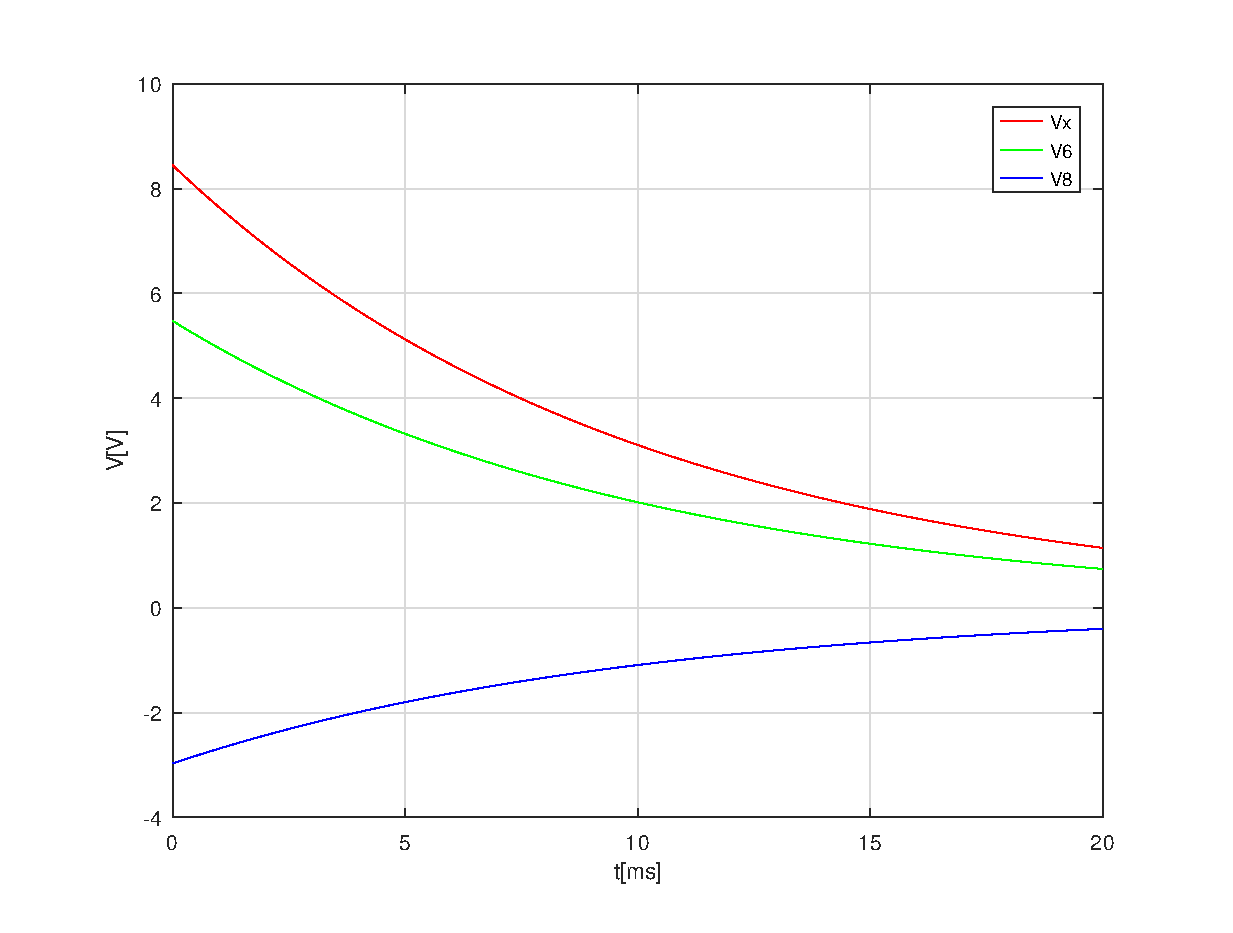
\includegraphics[width=0.8\linewidth]{Natural.eps}
    \caption{Natural response.}
    \label{fig:NatOc}
\end{figure}

 

\subsubsection{Transient analysis: Forced solution}
\indent

To find the forced solution, we used complex numbers in order to simplify the calculations. Every component of the circuit but the sources was substituted by a "black box" with the same impedance ($Z$), which can be calculated using equation \ref{eq:ImpR} (Phasor Ohm's Law) for resistors and equation \ref{eq:ImpC} for capacitors.

\begin{equation}
    Z_R=\frac{\widetilde{V}} {\widetilde{I}}=R\hspace{5pt},
    \label{eq:ImpR}
\end{equation}

\begin{equation}
    Z_C=\frac{1}{j \omega C} \hspace{5pt}.
    \label{eq:ImpC}
\end{equation}

The voltage source $V_s$ is now imposing a sinusoidal excitation on the circuit with a frequency ($f$) of $1KHz$, and therefore its voltage varies in time according to the wave equation \ref{eq:svs}.

\begin{equation}
    v(t)=Vcos(\omega t-\phi) \hspace{5pt}.
    \label{eq:svs}
\end{equation}

Knowing that $v_s(0)=0$, $V_s=1 V$ and that $w=2\pi f$, we find $v_s$'s phase ($\phi$) value which is $90^\circ$.

At last, we use the KCL (equation \ref{eq:KCL}) in every node possible as described in subsection \ref{subsection:circ_analysis}, computing the voltage in each node.

The voltage in this case is a complex number. By taking its absolute value we obtain the magnitude, while the phase is obtained by taking its argument. With both values computed, the plot for the voltages can be made according to the equation \ref{eq:svs}.


\begin{figure}[H] \centering
    \includegraphics[width=0.8\linewidth]{Forced.eps}
    \caption{Forced response.}
    \label{fig:ForOC}
\end{figure}



\begin{table}[H]
    \caption{Phase and magnitude of the voltage on each node}
    \begin{subtable}{.5\linewidth}
      \centering
        \caption{Magnitude}
        \begin{tabular}{ll}
        \hline    
        {\bf Name} & {\bf Value [V]} \\ \hline
        \input{../Analysis/Voltages_M.tex}
        \end{tabular}
        \label{tab:MagnitudeOc}
    \end{subtable}%
    \begin{subtable}{.5\linewidth}
      \centering
        \caption{Phase}
        \begin{tabular}{ll}
        \hline    
        {\bf Name} & {\bf Value [Degrees]} \\ \hline
        \input{../Analysis/Voltages_Ph.tex}
        \end{tabular}
        \label{tab:PhaseOc}
    \end{subtable} 
\end{table}

    
\subsubsection{Transient analysis: Final solution}

\indent

Since the natural and forced responses are already known, the final solution can be calculated simply by adding the natural and forced responses together. By doing this we obtain the following graph (Figure \ref{fig:FinalOc}):


\begin{figure}[H] \centering
    \includegraphics[width=0.8\linewidth]{FinalResponse.eps}
    \caption{Final response.}
    \label{fig:FinalOc}
\end{figure}


The voltages before the oscillating regime were also added to this graph, with the purpose of showing the boundary conditions.

\subsubsection{Frequency analysis}


\indent

By iterating what was made in previous subsections while changing the frequency, it was possible to analyse the frequency variation's impact on the magnitude and phase on each node. The outcome may be seen in figures \ref{fig:FreqMagOc} and \ref{fig:FreqPhOc}.


\begin{figure}[H] \centering
    \includegraphics[width=0.8\linewidth]{Magnitude.eps}
    \caption{Magnitude graph.}
    \label{fig:FreqMagOc}
\end{figure}



\begin{figure}[H] \centering
    \includegraphics[width=0.8\linewidth]{Phase.eps}
    \caption{Phase graph.}
    \label{fig:FreqPhOc}
\end{figure}
